\graphicspath{{content/summary/figures/}}

\section{Overview}

%TODO might want to rephrase this. The following two facts are relevant.


This thesis will introduce a new tool that can automatically fix data-races in
Java programs. There are two relevant facts of software engineering that are the
basis of the motivation behind the tool:
\begin{enumerate}
  \item software engineers have had to manage, arguably, the most complex
  systems ever built by humans for decades now.
  
  \item the software development community has been relying on Moore's Law
  to help improve the performance of their software since its beginning. But
  nowadays hardware performance boosting has shifted from higher CPU speed
  towards multiple processing units working in parallel.
\end{enumerate}

In order to handle the above mentioned complexity programmers have developed
numerous methods to help cope with it, one of which is \emph{refactoring}
(behaviour preserving transformations performed on the code). In recent years
many of these refactorings have been automated and all major IDEs offer
user-friendly support for these transformations, especially for code written in
the Java language. The automation of refactorings, in turn, reveals an
interesting concept: the separation of roles in human-machine interaction.The
human is responsible for the consistency of the abstract, high-level concerns of
the system, while the machine performs the tedious and repetitive analyses and
transformations necessary for performing refactorings.

Furthermore, the difficulties raised by trying to make code execute
\emph{correctly} in parallel are non-trivial; add this to the fact that standard
software systems are in of themselves hard to manage, retrofitting old software
to this new paradigm becomes a very difficult problem. One of the most common
issue in parallel programs are data races; a data race arises when two different
threads contend for the same data, one with a write access the other one with a
read access.

\paragraph{From the two points above}an obvious idea comes to mind: a tool that
helps the programmer transform sequential code into parallel code; thus freeing
the programmer from the burden of the tedious transformations done on legacy
systems whose performance no longer improves with new hardware.
Such a tool exists in the form of ReLooper~\cite{ReLooper}. Briefly described,
ReLooper takes as input a user-selected loop that performs computationally
intensive operations on large data sets and converts it using Java's
\emph{ParalelArray} data structure which facilitates easy execution of parallel
tasks on the array's elements. This transformation can be performed only if the
code that comprises these tasks does not result in any data-races in the context
of parallel execution.

\paragraph{Our tool}comes as a natural extension to ReLooper in the sense that
it attempts to solve such data-races. But, data-races can manifest themselves in
multiple ways so we used a best practice when it comes to automated
refactoring tools: identifying the most common changes that are
executed in a consistent manner in real world software systems, in order have
the greatest impact on programmer productivity. Thus, we started out by
analyzing a total of 34 open-source Java projects (out of which 3 were viable
candidates for parallelization). We realized that we had to make one particular
change over and over again. Namely, make data that was once shared between
threads unique to each one; every thread getting its own copy of the data. There
are two ways of doing this: 
\begin{enumerate} 
  \item [a)] move object allocation to the parallel context. Identify whether or
  not this is possible is a non-trivial problem. 
  \item [b)] encapsulate objects in Java's \emph{ThreadLocal}, a wrapper class
  that ensures that the data enclosed is unique for each thread. A sequential
  program executed using ThreadLocal objects behaves the same as the old
  version, but it also ensures that when executed concurrently each thread
  receives its own copy of the data, all at the cost of some overhead
  introduced by \emph{ThreadLocal} itself. To show that this overhead is not
  negligible we did the following: in the case of Jmol~\cite{Jmol-site}, we
  simply refactored each individual field that was involved in a race (34
  fields) to be \emph{ThreadLocal}. The difference in performance is from an
  average sequential running time of 1.4s to 2.2s; so an overhead of roughly
  63\%.
\end{enumerate}

An abstract overview of the major computational tasks that our tool does in
order to perform the above mentioned transformation can be seen in
Figure~\ref{algo}.

\begin{figure}[h!]
\begin{center}
  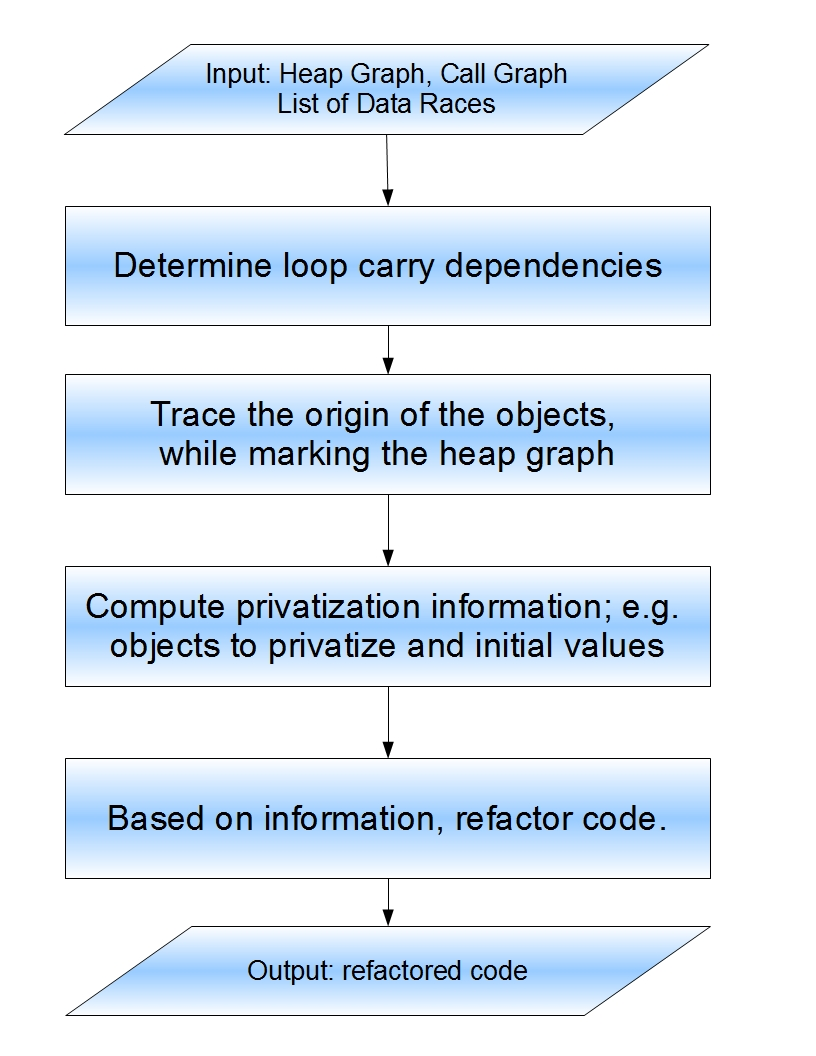
\includegraphics[width=7cm]{algo}
  \caption{Flow chart coarsely describing the tool}
  \label{algo}
\end{center}
\end{figure}

We dubbed the transformations described above as \emph{data privatization},
which will be the term we will use hereafter. This thesis will focus mostly on
the second method, but with slight variations. Instead of \emph{ThreadLocal} we use
our own construct called \emph{ThreadPrivate} which behaves mostly like
\emph{ThreadLocal}, but it offers more robust support for ensuring that the
copy of the data that is referenced in each of the threads is in the proper
state (i.e. the one it is in right before the execution of the parallel operation).


\paragraph{A very important} precondition that has to be met is that the data is
not involved in a particular type of data-race that we call a \emph{loop carried
dependency}. Basically the fields must not be used as temporary storage between
the iterations of the loop. Reliably determining whether or not a data-race is a
\emph{loop carried dependency} has proven to be the most challenging task in
building this tool. It requires a complex analysis of the control flow graph
obtained through static analysis of the Java source code.
Because of the fact that the detection of loop carried dependencies was at that
point in time an unsolved problem we've had to go through several failed
attempts before we've concluded that it is basically an \emph{interprocedural,
finite, distributive, subset (IFDS) problem}~\cite{IFDS}. Luckily,
WALA~\cite{wala-site}, the static analysis library we used offered support for
solving these kinds of problems and we came up with a very elegant and compact
solution that works with 100\% accuracy; as opposed to the previously verbose
and inaccurate solutions.

\paragraph{After determining} which of the fields can be safely privatized we
trace their origin. We do that using a graph algorithm that traverses the heap
graph by going through the def-uses of the field in question. The trace is
limited to the context of the parallel loop operator because we care only about
the last owner of the objects at the start of the parallel context. This last
owner is the one that will be the target of the refactoring.

\paragraph{Last,}the information gathered during the origin trace is used to
compute the privatization scheme which aims to minimize the overhead introduced by
\emph{ThreadPrivate}. This privatization scheme is used by our refactoring
(built on top of the eclipse IDE) to perform the necessary transformations.

\section{Implementation}
The bulk of the complexity of our project is theoretical, once we managed to
solve these issues the implementation of the tool itself became simple. We
encountered no noteworthy engineering difficulties, our tool comprising of
roughly 6000 lines of code distributed over 30 classes, the interaction between
these is simple and very comprehensible.

But to give you an idea on the of the amount of work we put into the initial
phase of analysing open-source projects, to do the first manual parallelization
of Jmol we had to:
\begin{itemize}
  \item run the program with a the YourKit Java profiler~\cite{YourKit}in order
  to find computationally intensive loops.
  \item analyze 101 fields distributed over 6 classes, that were reference a
  total of 997 times in the future parallel context to check for data-races
  \item privatize the 34 fields that were proven to be data-races using
  \emph{ThreadLocal}
  \item the privatization led the update of 359 field references due to the
  indirection introduced by \emph{ThreadLocal}
\end{itemize}

\section{Conclusions}

\paragraph{In conclusion,} this thesis proposes a novel solution for a fairly
common problem encountered when trying to retrofit sequential code to parallel
code and it presents an experimental tool that is able to successfully perform
these transformations on sandbox versions of the analyzed projects (i.e.
reduced programs to only a few tens of thousands of lines of code). But the
novel theoretical issue of determining loop carried dependencies is,
potentially, a useful contribution to future race-detection or parallel
correctness verification tools.
